\documentclass[12pt, a4paper, oneside, fontset=windows]{ctexart}
\usepackage{amsmath, amsthm, amssymb, appendix, bm, graphicx, hyperref, mathrsfs,listings,xcolor}

\title{\textbf{大数据管理方法与应用第二次作业}}
\author{大数据001\\郅啸淇\\学号:2184114639}
\date{\today}
\linespread{1.5}
\lstset{
    basicstyle          =   \sffamily,          % 基本代码风格
    keywordstyle        =   \bfseries,          % 关键字风格
    commentstyle        =   \rmfamily\itshape,  % 注释的风格,斜体
    stringstyle         =   \ttfamily,  % 字符串风格
    flexiblecolumns,                % 别问为什么,加上这个
    numbers             =   left,   % 行号的位置在左边
    showspaces          =   false,  % 是否显示空格,显示了有点乱,所以不现实了
    numberstyle         =   \zihao{-5}\ttfamily,    % 行号的样式,小五号,tt等宽字体
    showstringspaces    =   false,
    captionpos          =   t,      % 这段代码的名字所呈现的位置,t指的是top上面
    frame               =   lrtb,   % 显示边框
}

\lstdefinestyle{Python}{
    language        =   Python, % 语言选Python
    basicstyle      =   \zihao{-5}\ttfamily,
    numberstyle     =   \zihao{-5}\ttfamily,
    keywordstyle    =   \color{blue},
    keywordstyle    =   [2] \color{teal},
    stringstyle     =   \color{magenta},
    commentstyle    =   \color{red}\ttfamily,
    breaklines      =   true,   % 自动换行,建议不要写太长的行
    columns         =   fixed,  % 如果不加这一句,字间距就不固定,很丑,必须加
    basewidth       =   0.5em,
}
\lstdefinestyle{Matlab}{
    language        =   Matlab, % 语言选Matlab
    basicstyle      =   \zihao{-5}\ttfamily,
    numberstyle     =   \zihao{-5}\ttfamily,
    keywordstyle    =   \color{blue},
    keywordstyle    =   [2] \color{teal},
    stringstyle     =   \color{magenta},
    commentstyle    =   \color{red}\ttfamily,
    breaklines      =   true,   % 自动换行,建议不要写太长的行
    columns         =   fixed,  % 如果不加这一句,字间距就不固定,很丑,必须加
    basewidth       =   0.5em,
}
\newtheorem{theorem}{定理}[section]
\newtheorem{definition}[theorem]{定义}
\newtheorem{lemma}[theorem]{引理}
\newtheorem{corollary}[theorem]{推论}
\newtheorem{example}[theorem]{例}
\newtheorem{proposition}[theorem]{命题}
\begin{document}
\maketitle
\newpage
%\tableofcontents
\newpage
\section{鸢尾花数据集降维}
\subsection{代码思路}
首先导入Iris数据集,然后使用PCA方法进行降维,保留三个主成分,最后使用Axes3D进行绘图,如图1所示。

\begin{figure}[h]
    \centering
    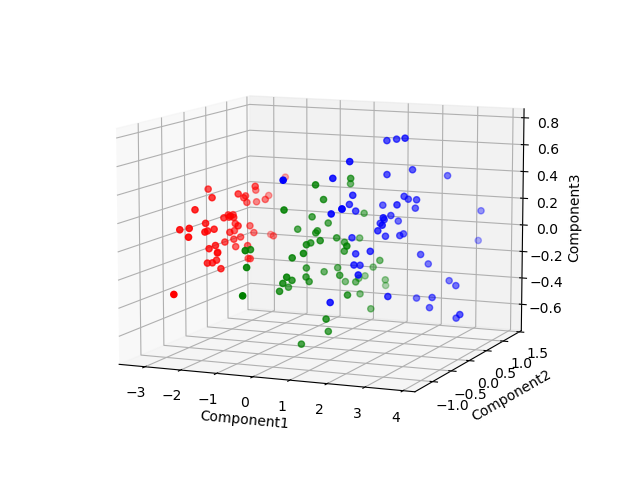
\includegraphics[scale = 0.8]{3D_Iris.png}
    \caption{降维后鸢尾花数据集}
\end{figure}
\subsection{完整代码}
\lstinputlisting[style = Python]{Iris_PCA.py}

\section{手写体数据集降维分类}
\subsection{代码思路}
首先不使用PCA对数据降维,直接使用SVM进行分类,得出正确率为0.9867,使用PCA压缩保留前32个主成分(原图片为8*8,共64个维度),得到新的分类正确率为0.5089
\subsection{完整代码}
\lstinputlisting[style = Python]{Digits_SVM.py}
\section{PCA压缩图片}
\subsection{代码思路}
首先使用PIL读入图片,原图片如图2所示,其分辨率为555*377,接着将每一行视作一个特征,使用PCA分别保留1\%,2\%,5\%,10\%,20\%,30\%,如图3,4,5,6,7,8所示,可以看出保留比例越大图像效果越接近原图。
\begin{figure}[htbp]
    \centering
    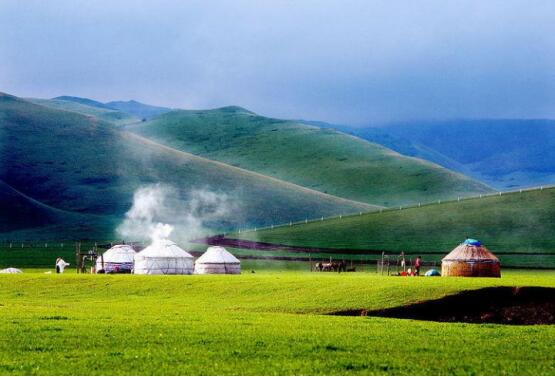
\includegraphics[scale = 0.5]{test.jpg}
    \caption{原图}
\end{figure}
\begin{figure}[htbp]
    \centering
    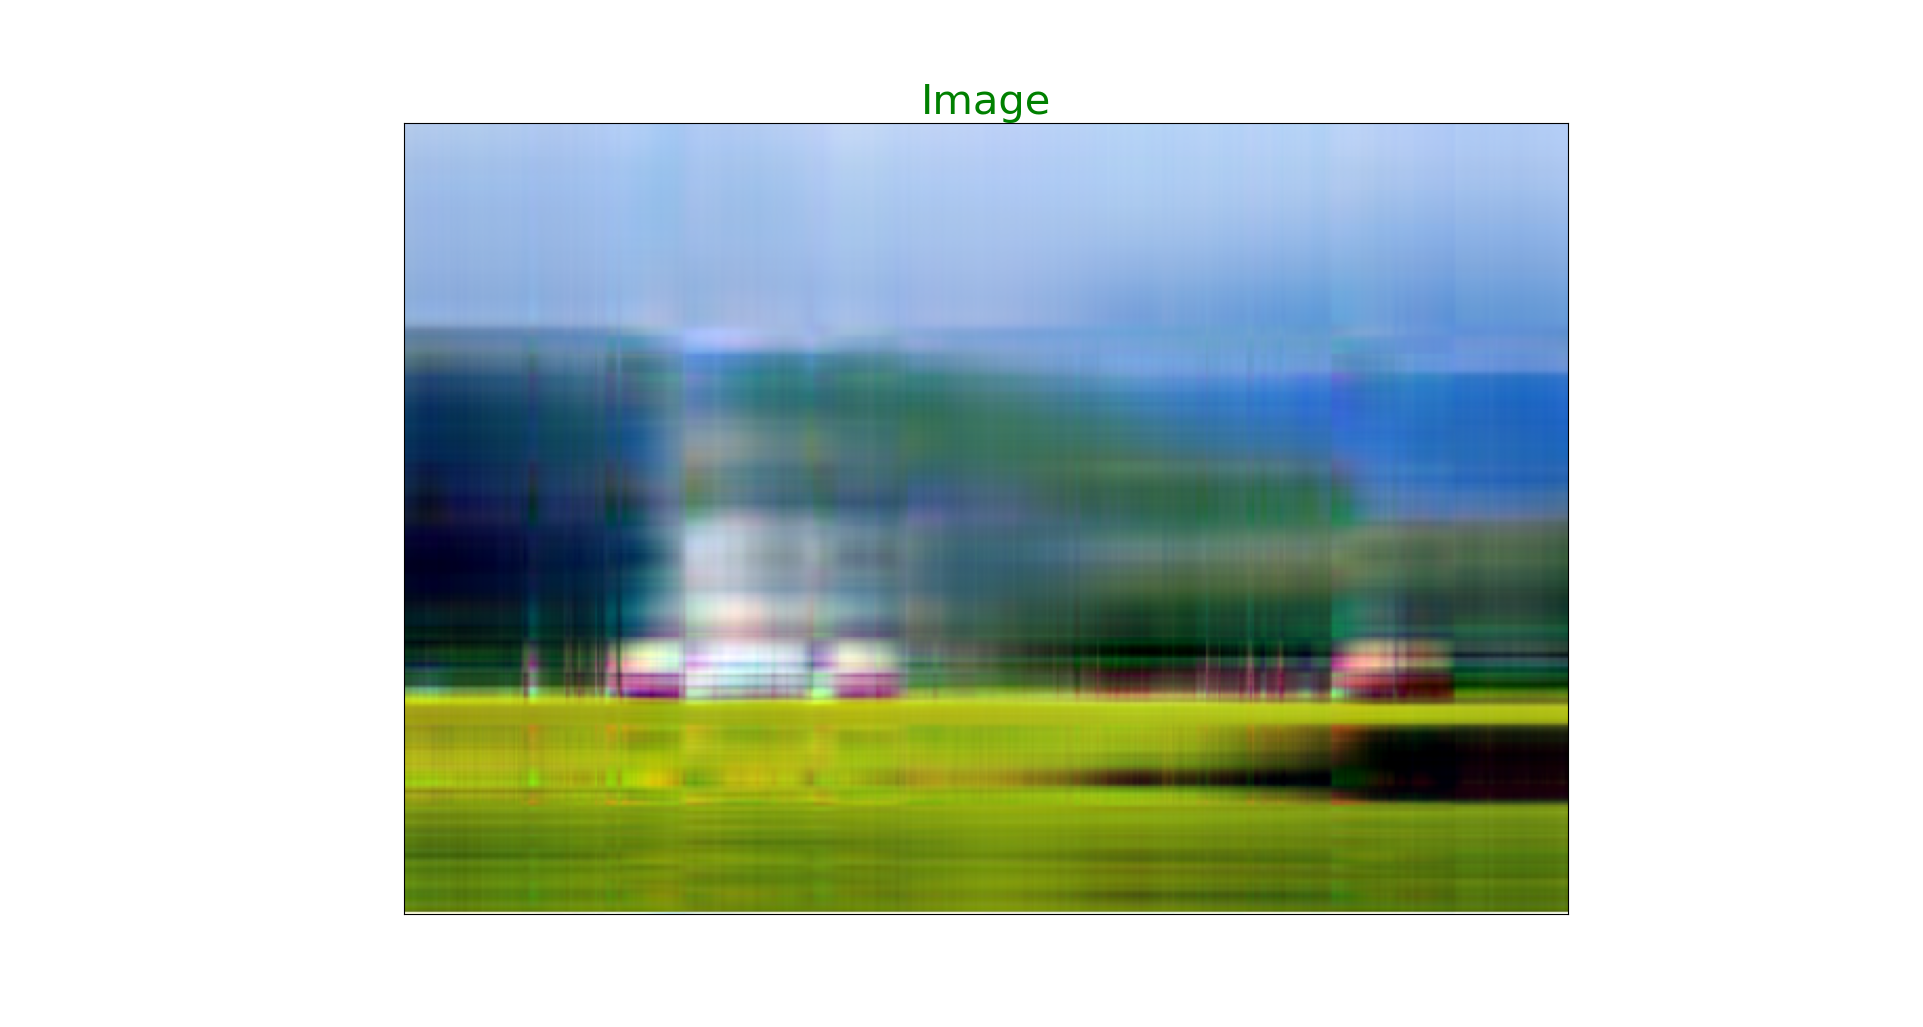
\includegraphics[scale = 0.3]{1.png}
    \caption{保留1\%}
\end{figure}
\begin{figure}[htbp]
    \centering
    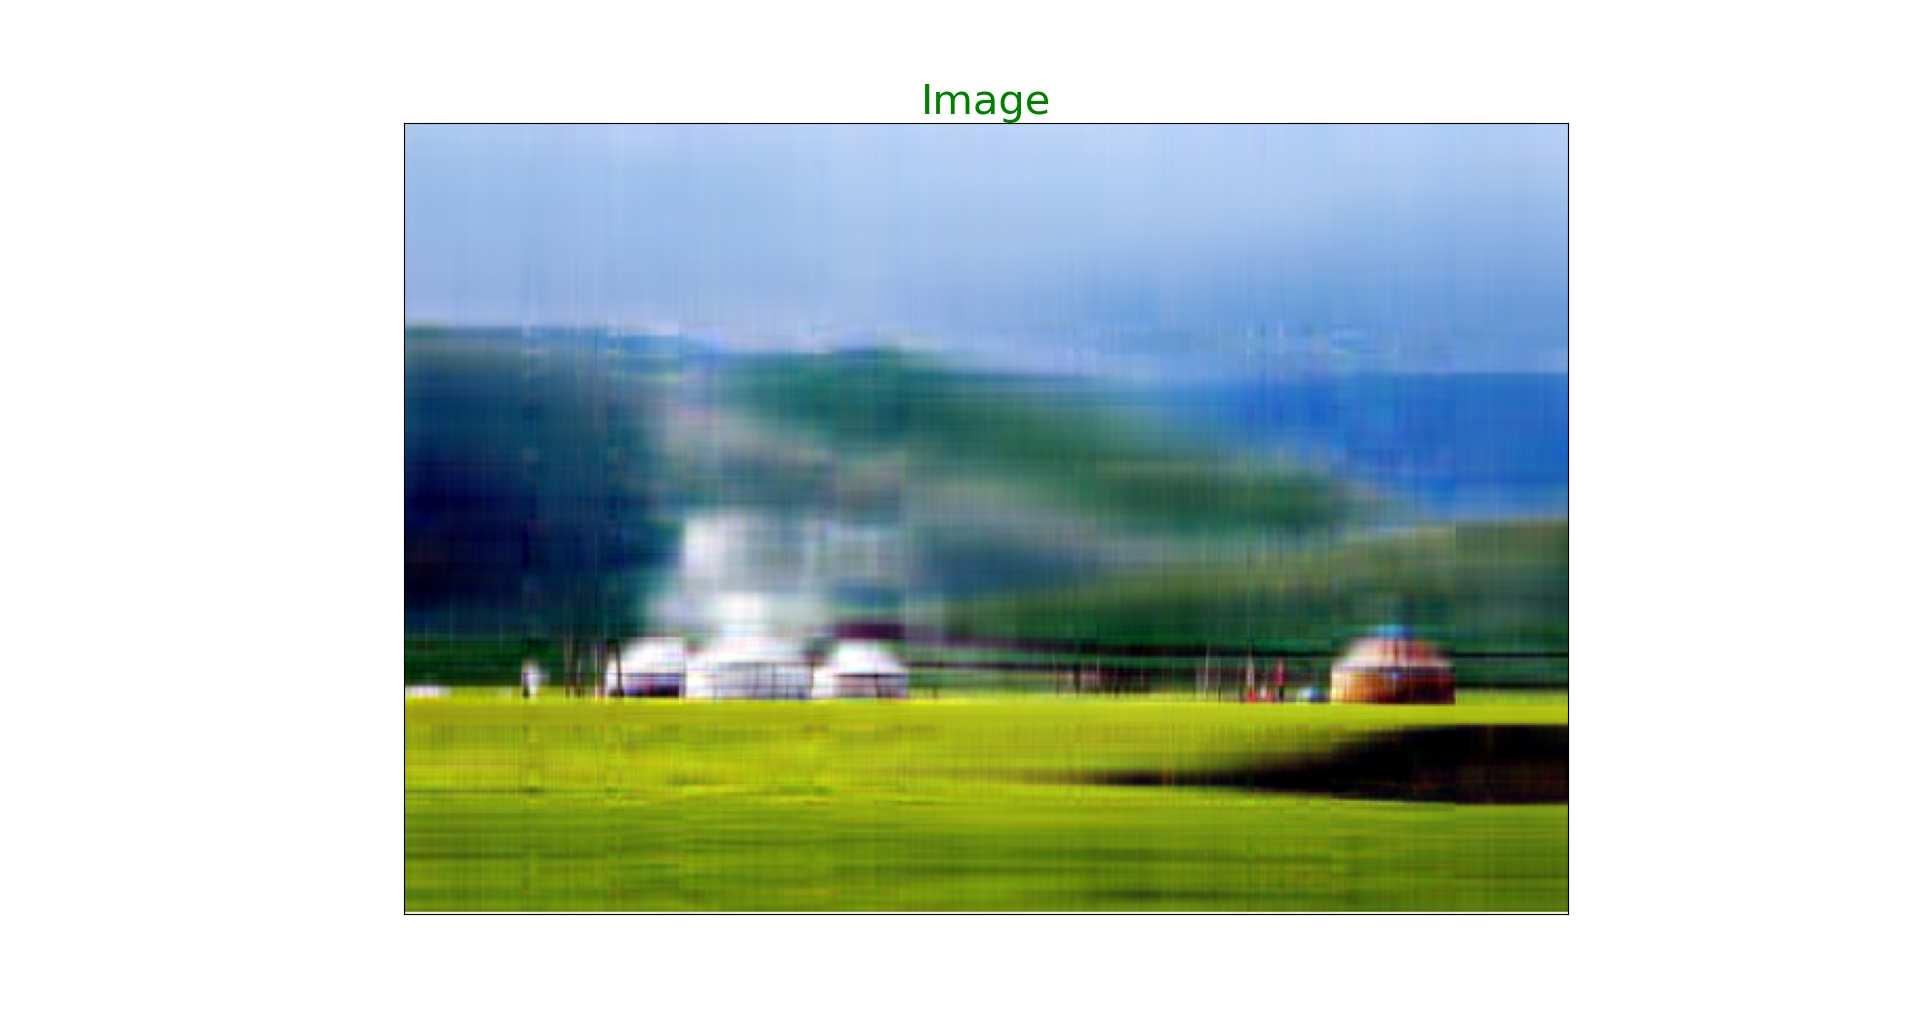
\includegraphics[scale = 0.3]{2.png}
    \caption{保留2\%}
\end{figure}
\begin{figure}[htbp]
    \centering
    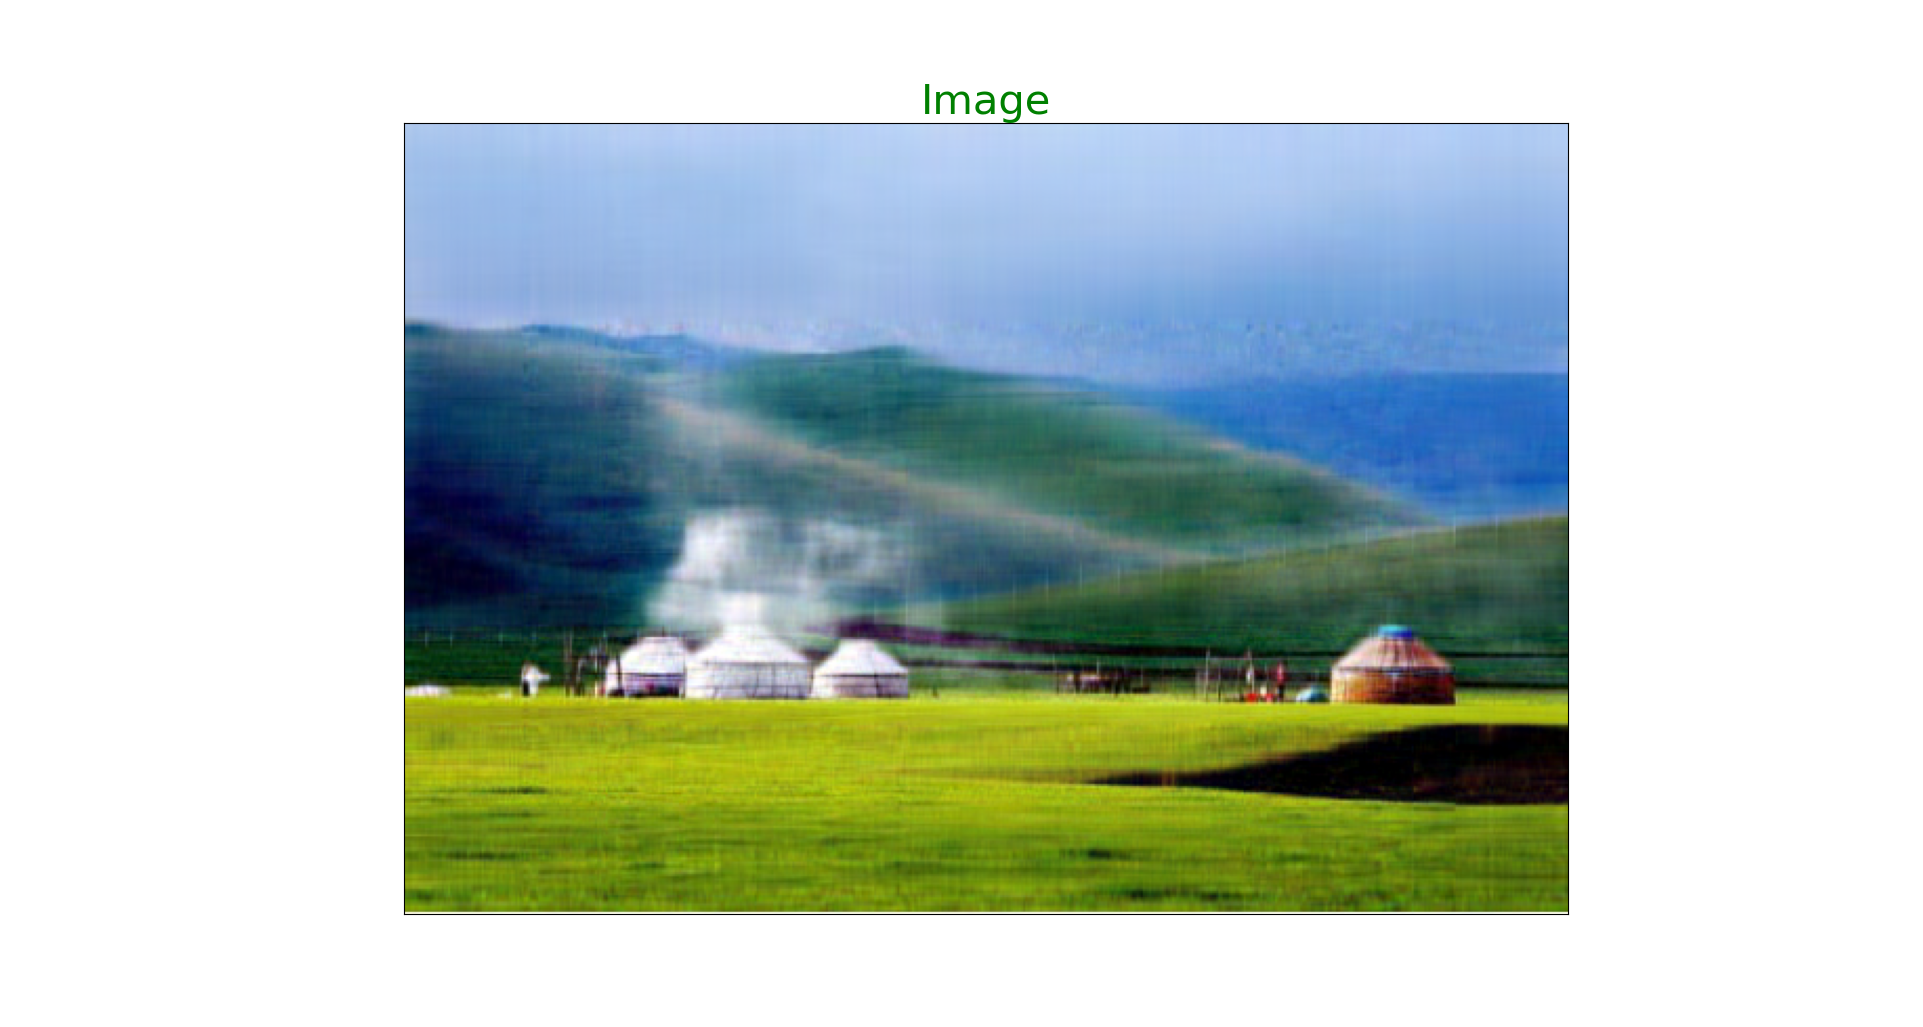
\includegraphics[scale = 0.3]{5.png}
    \caption{保留5\%}
\end{figure}
\begin{figure}[htbp]
    \centering
    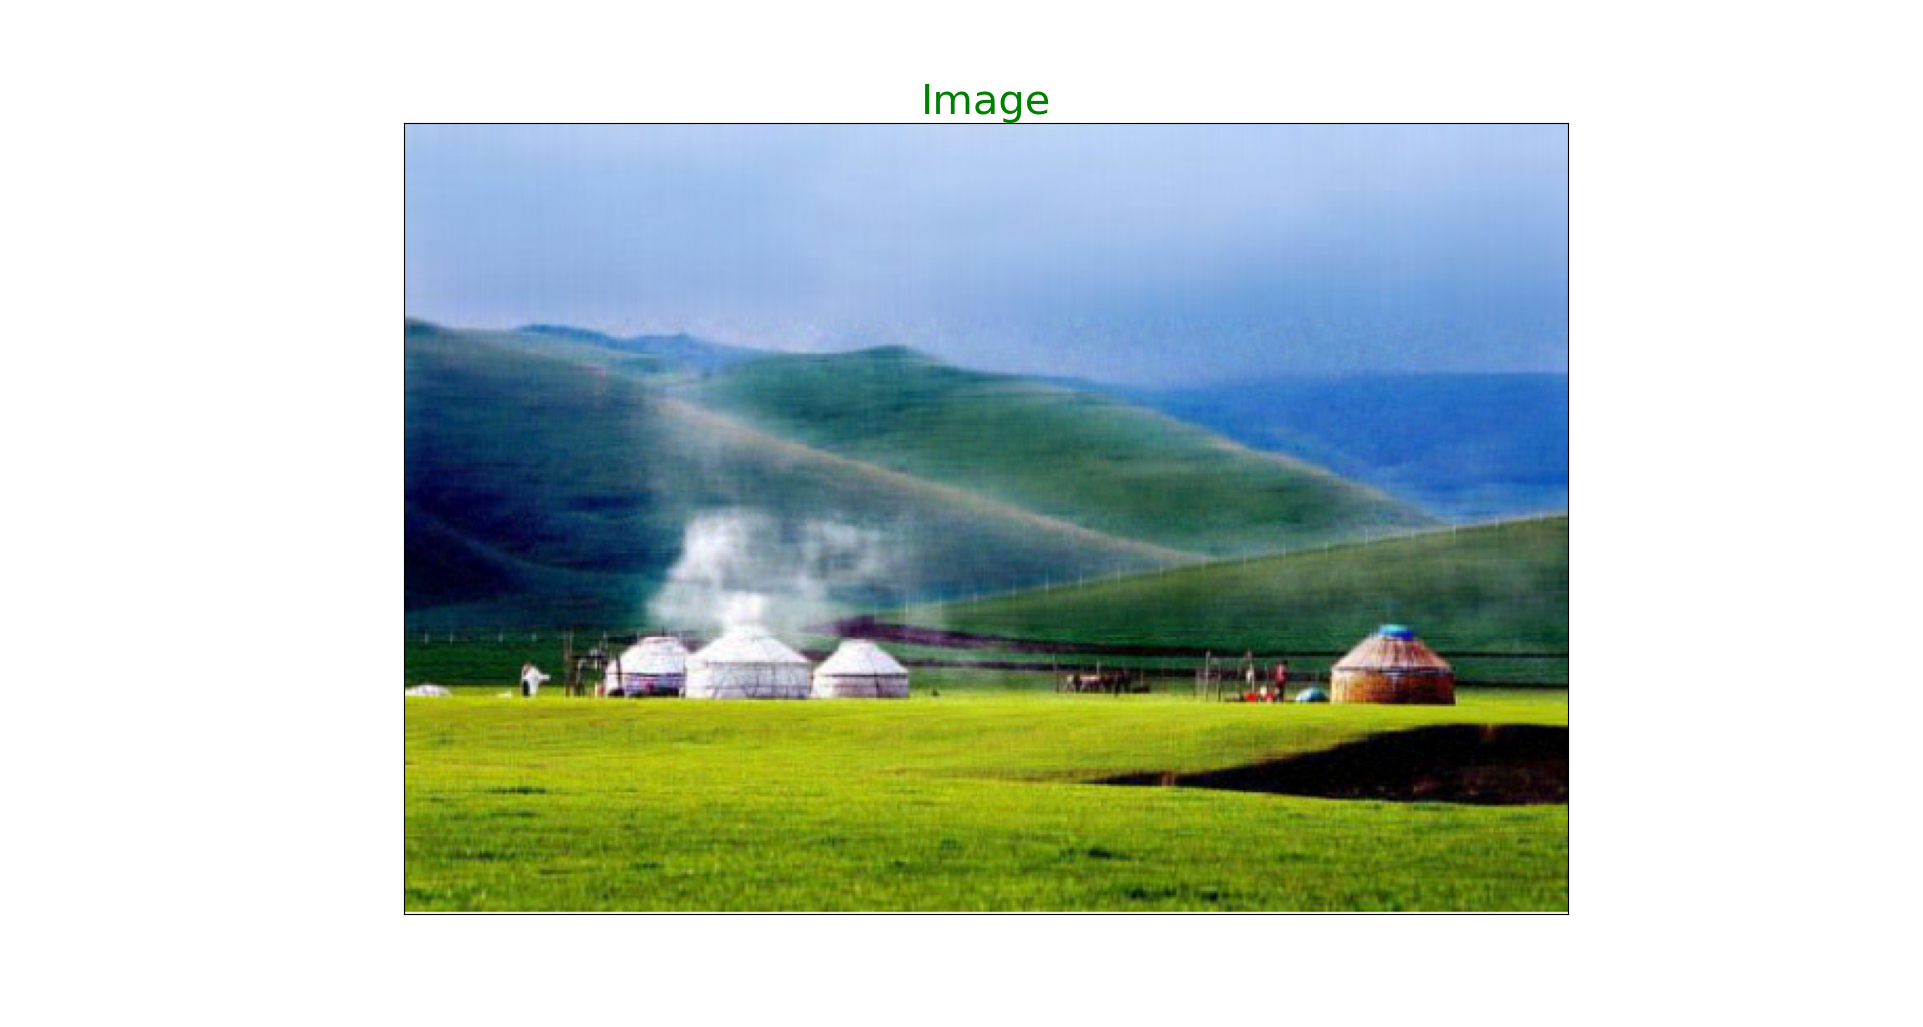
\includegraphics[scale = 0.3]{10.png}
    \caption{保留10\%}
\end{figure}
\begin{figure}[htbp]
    \centering
    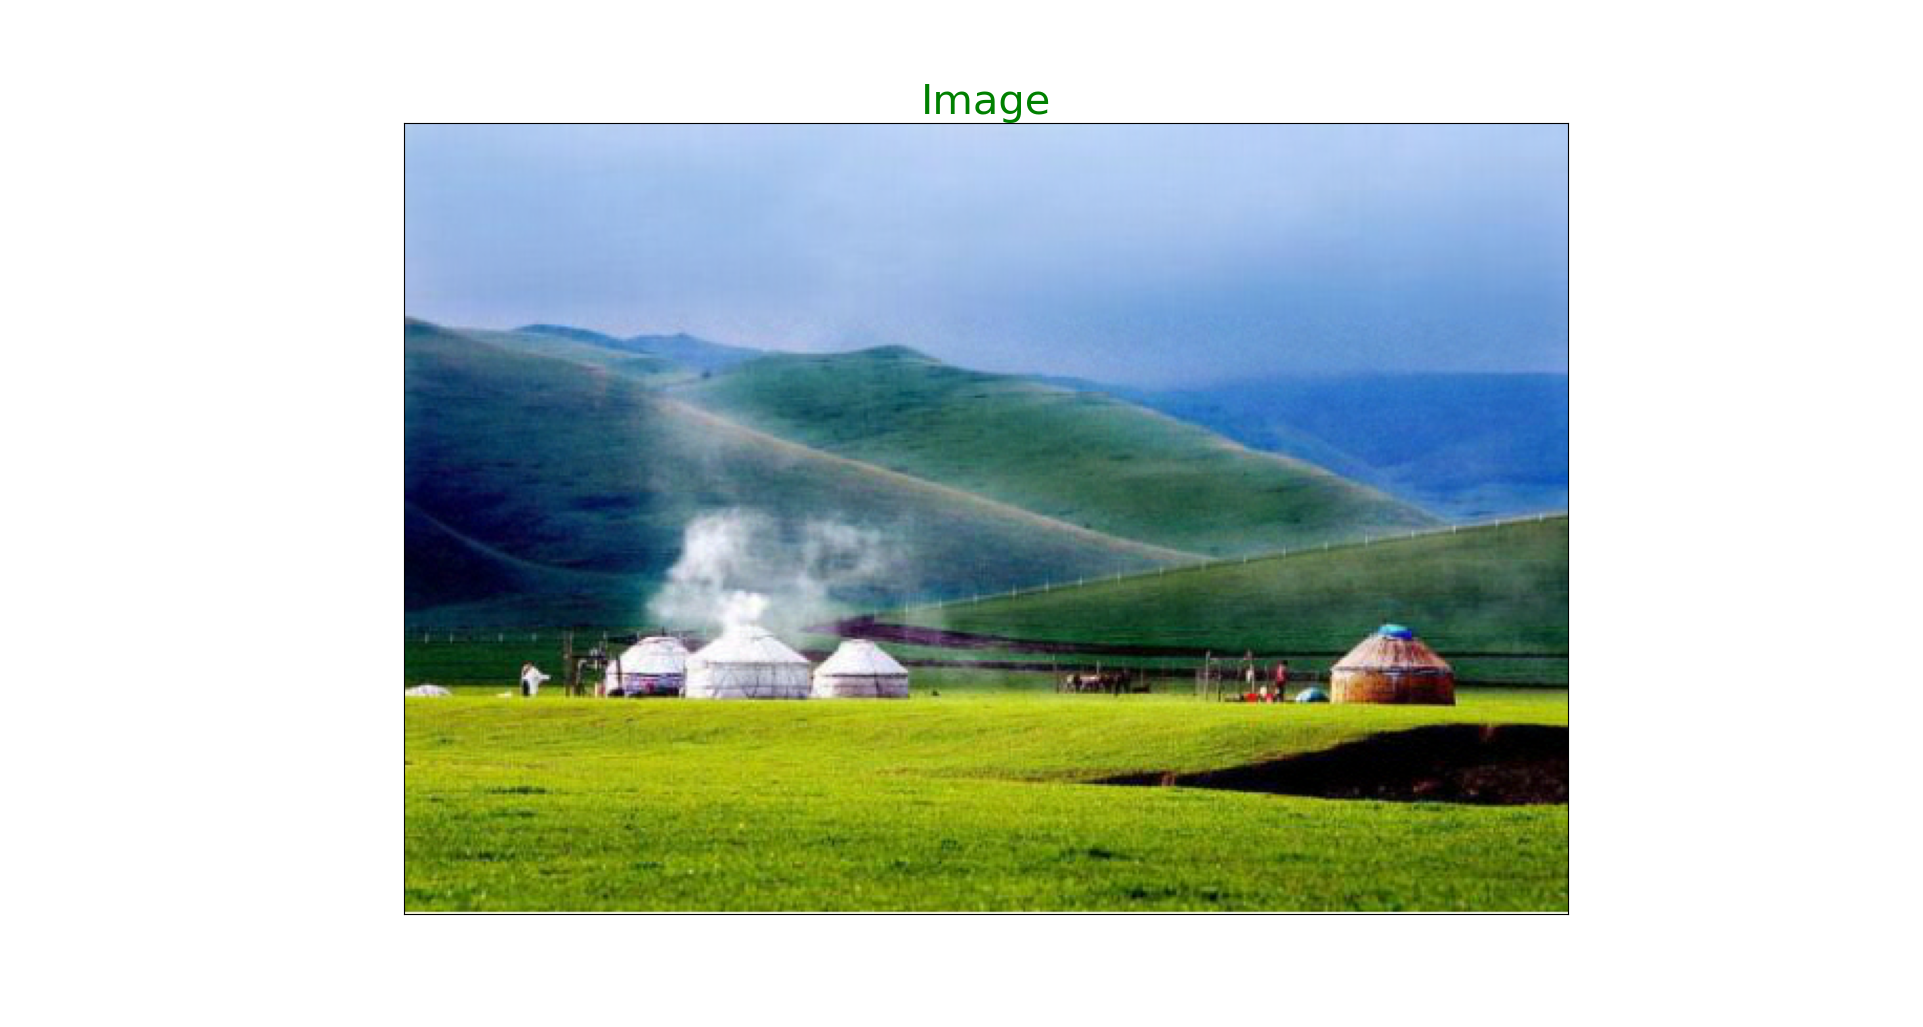
\includegraphics[scale = 0.3]{20.png}
    \caption{保留20\%}
\end{figure}
\begin{figure}[htbp]
    \centering
    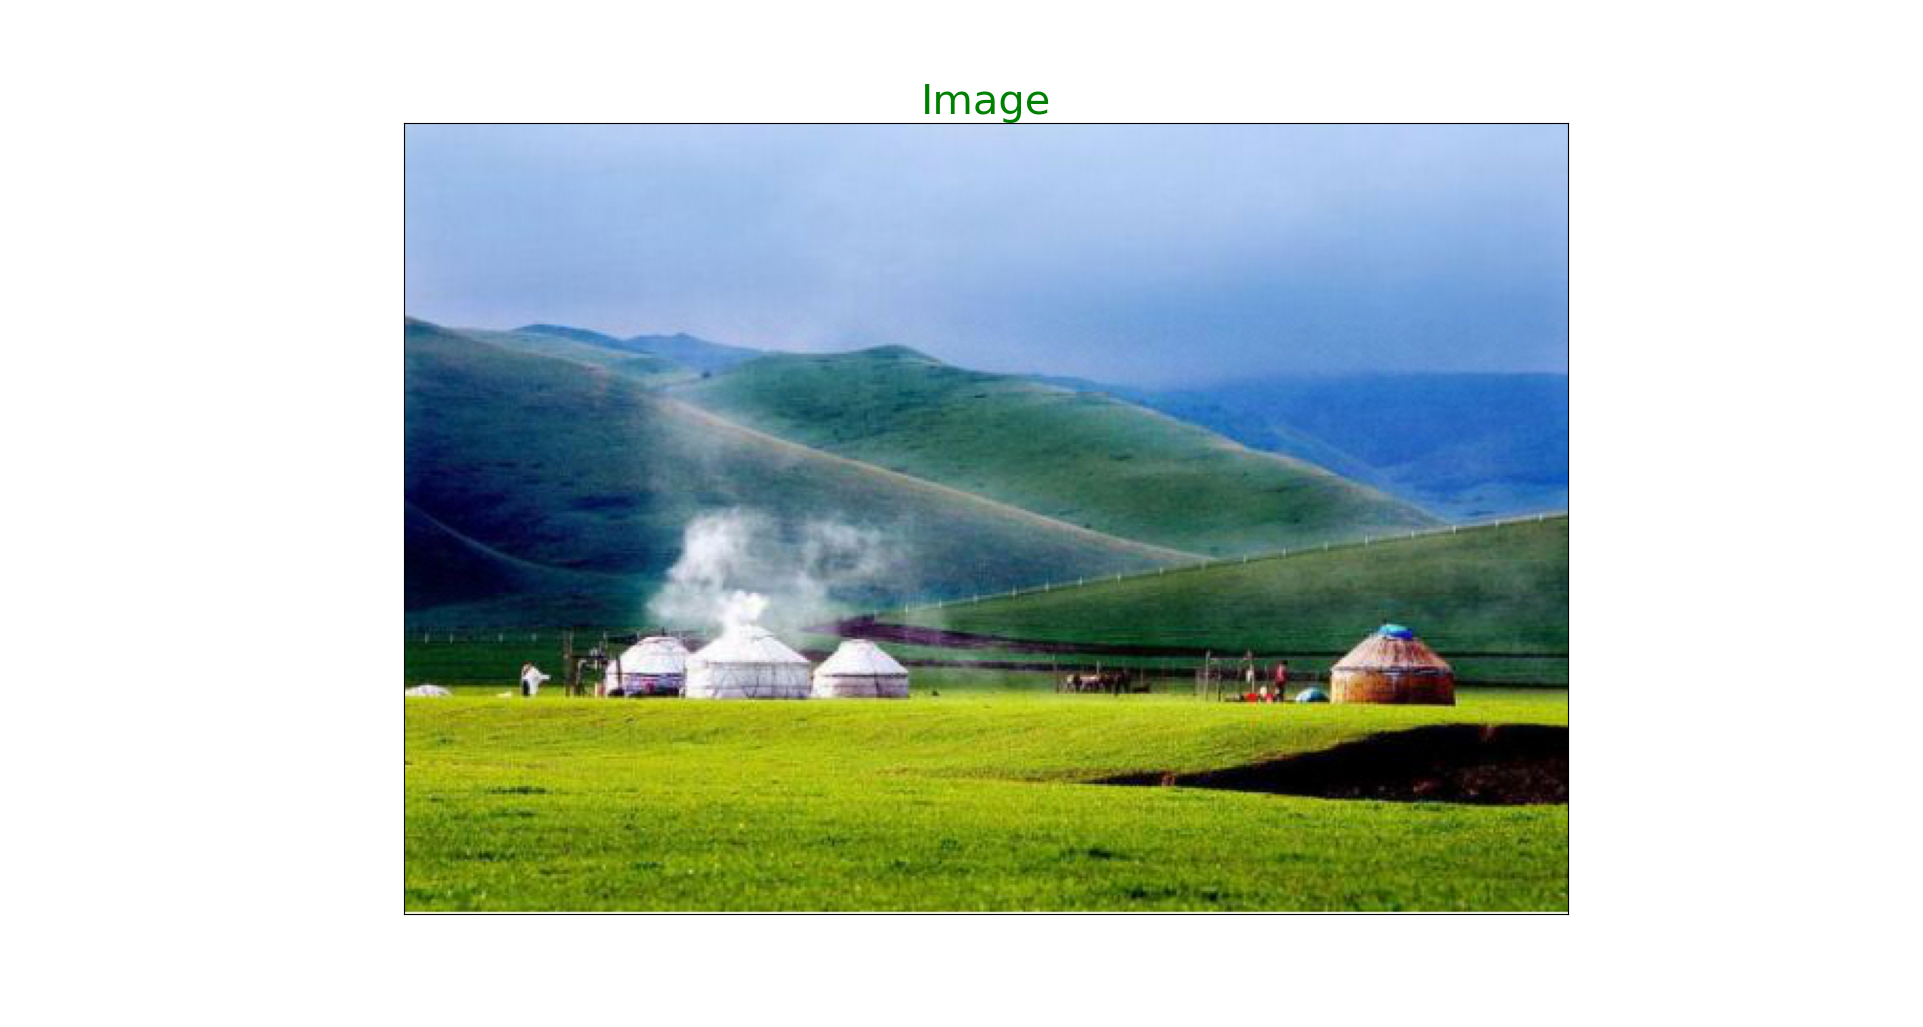
\includegraphics[scale = 0.3]{30.png}
    \caption{保留30\%}
\end{figure}
\newpage
\subsection{完整代码}
\lstinputlisting[style = Python]{PCA_Image.py}
\section{人脸识别数据集降维分类}
\subsection{代码思路}
首先读取fetch\_lfw\_people数据集,直接使用SVM进行分类,正确率为0.80,然后使用PCA方法保留前150个主成分,再进行SVM分类,正确率降低为0.77,同时提取出前十二个权重最大的主成分并绘图,得到权重排名前十二的特征脸,如图9所示。
\begin{figure}[htbp]
    \centering
    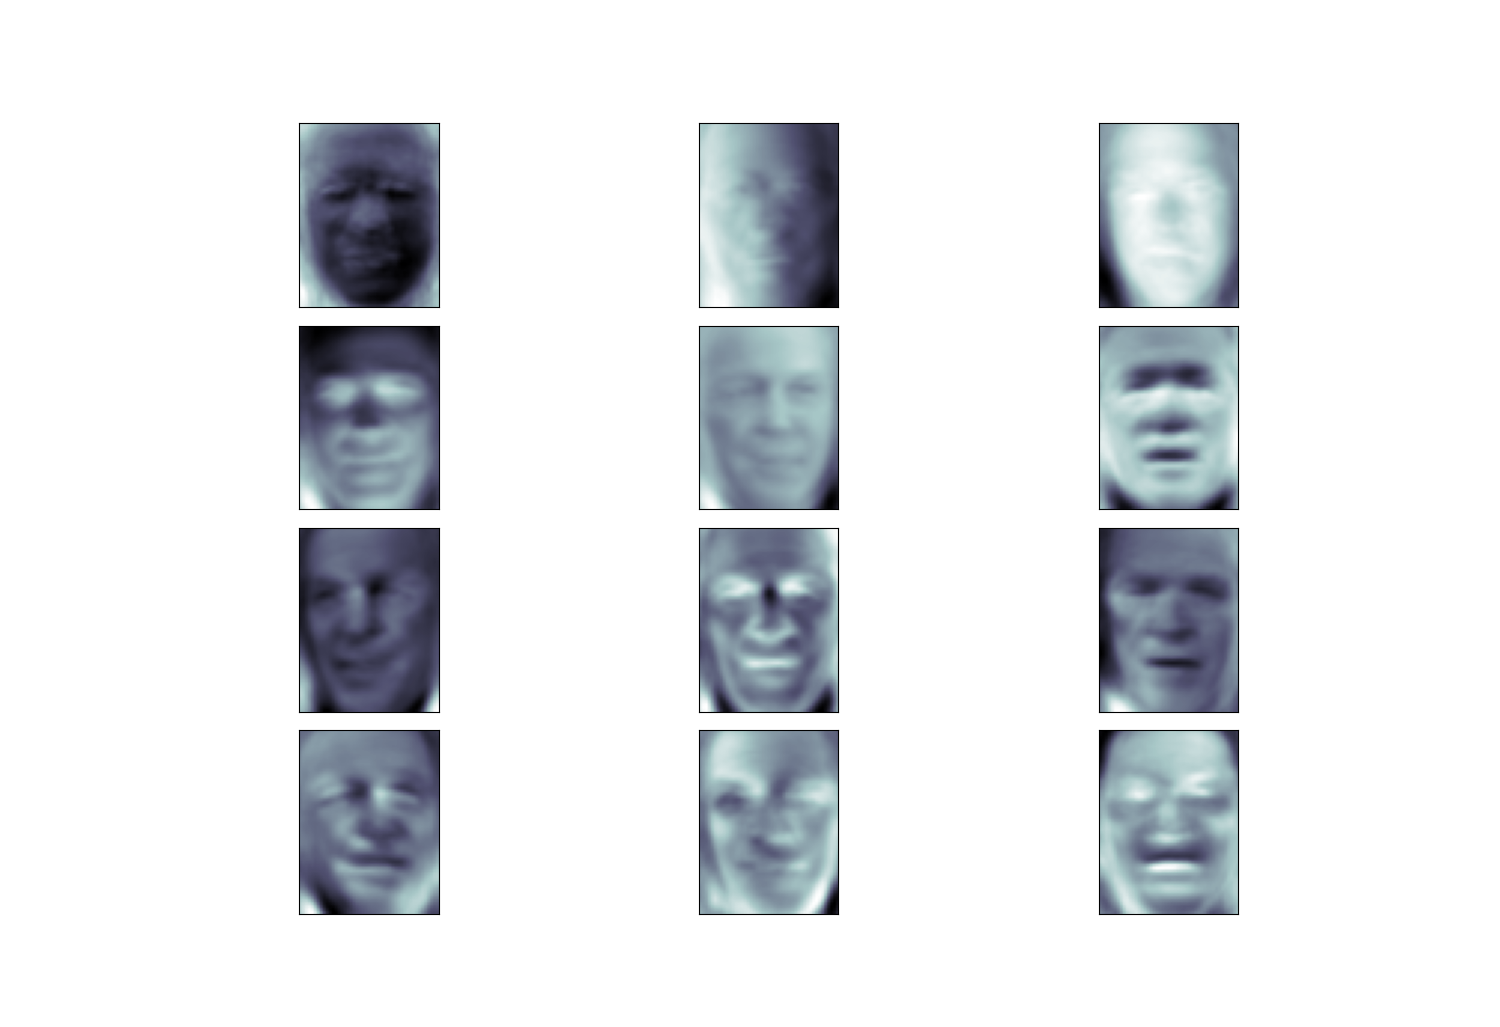
\includegraphics[scale = 0.3]{feature_face_TOP12.png}
    \caption{权重排名前十二的特征脸}
\end{figure}
\newpage
\subsection{完整代码}
\lstinputlisting[style = Python]{fetch_lfw_people_SVM.py}
\end{document} 